\section{Line fitting, residuals, and correlation}

%%%%%%%%%%%%%%%%%%%%%%%%%%%%%%%%%%%%

\begin{frame}
\frametitle{Modeling numerical variables}

In this unit we will learn to quantify the relationship between two numerical variables, as well as modeling numerical response variables using a numerical or categorical explanatory variable.

\end{frame}

%%%%%%%%%%%%%%%%%%%%%%%%%%%%%%%%%%%%

\begin{frame}
\frametitle{Poverty vs. HS graduate rate}

The \hl{scatterplot} below shows the relationship between HS graduate rate in all 50 US states and DC and the \% of residents who live below the poverty line {\small (income below \$23,050 for a family of 4 in 2012)}.

\twocol{0.55}{0.45}{
\begin{center}
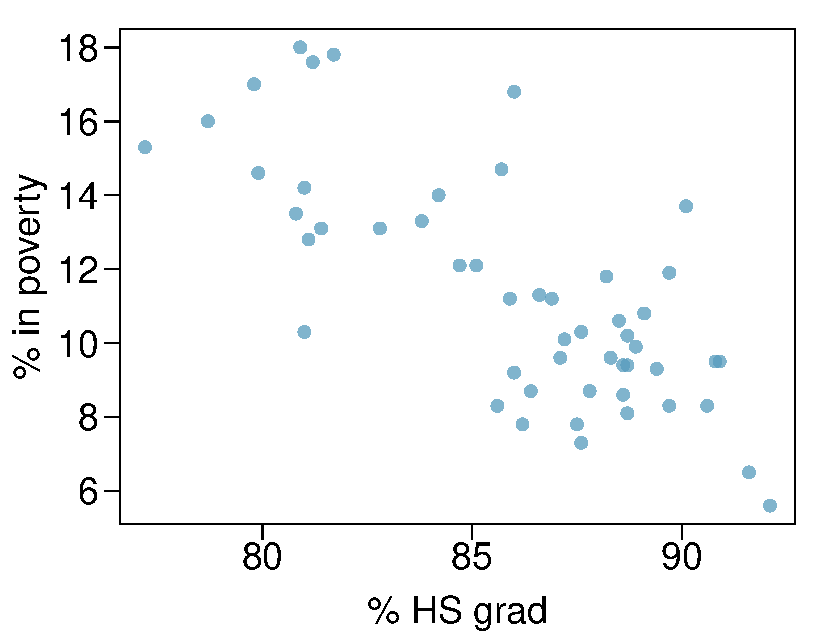
\includegraphics[width=\textwidth]{7-1_linefit_res_corr/figures/poverty/poverty_hsgrad}
\end{center}
}
{
\dq{Response variable?}
\pause
\soln{\% in poverty}
\pause
\dq{Explanatory variable?}
\pause
\soln{\% HS grad}
\pause
\dq{Relationship?}
\pause
\soln{linear, negative, moderately strong}
}

\end{frame}

%%%%%%%%%%%%%%%%%%%%%%%%%%%%%%%%%%%

\begin{frame}
\frametitle{Quantifying the relationship}

\begin{itemize}

\item \hl{Correlation} describes the strength of the \red{linear} association between two variables.

\pause

\item It takes values between -1 (perfect negative) and +1 (perfect positive).

\pause

\item A value of 0 indicates no linear association.

\end{itemize}

\end{frame}

%%%%%%%%%%%%%%%%%%%%%%%%%%%%%%%%%%%

\begin{frame}
\frametitle{Guessing the correlation}

\pq{Which of the following is the best guess for the correlation between \% in poverty and \% HS grad?}
\twocol{0.4}{0.6}
{
\begin{enumerate}[(a)]
\item 0.6
\solnMult{-0.75}
\item -0.1
\item 0.02
\item -1.5
\end{enumerate}
}
{
\begin{center}
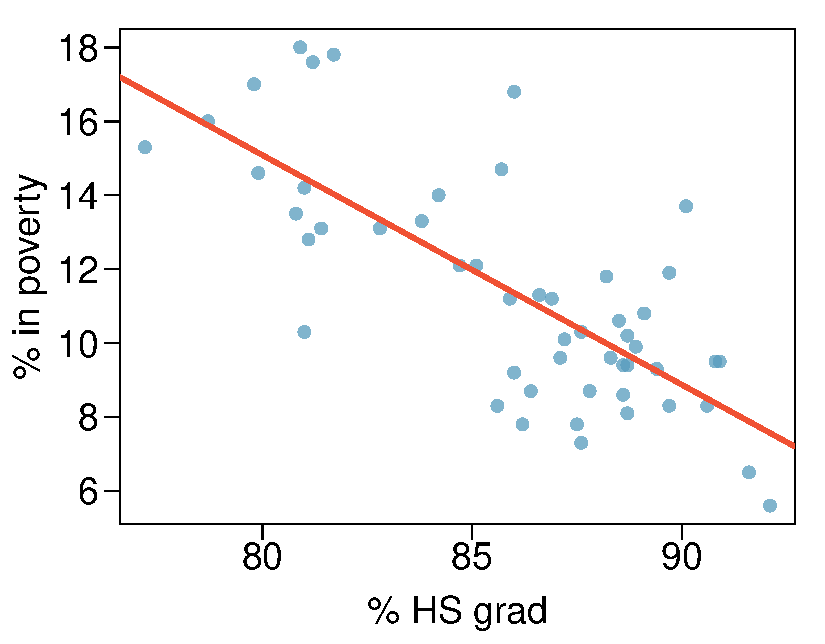
\includegraphics[width=\textwidth]{7-1_linefit_res_corr/figures/poverty/poverty_hsgrad_line}
\end{center}
}

\end{frame}

%%%%%%%%%%%%%%%%%%%%%%%%%%%%%%%%%%

\begin{frame}
\frametitle{Guessing the correlation}

\pq{Which of the following is the best guess for the correlation between \%~femail householder, no husband prsent and \%in poverty?}

\twocol{0.4}{0.6}
{
\begin{enumerate}[(a)]
\item 0.1
\item -0.6
\item -0.4
\item 0.9
\solnMult{0.5}
\end{enumerate}
}
{
\begin{center}
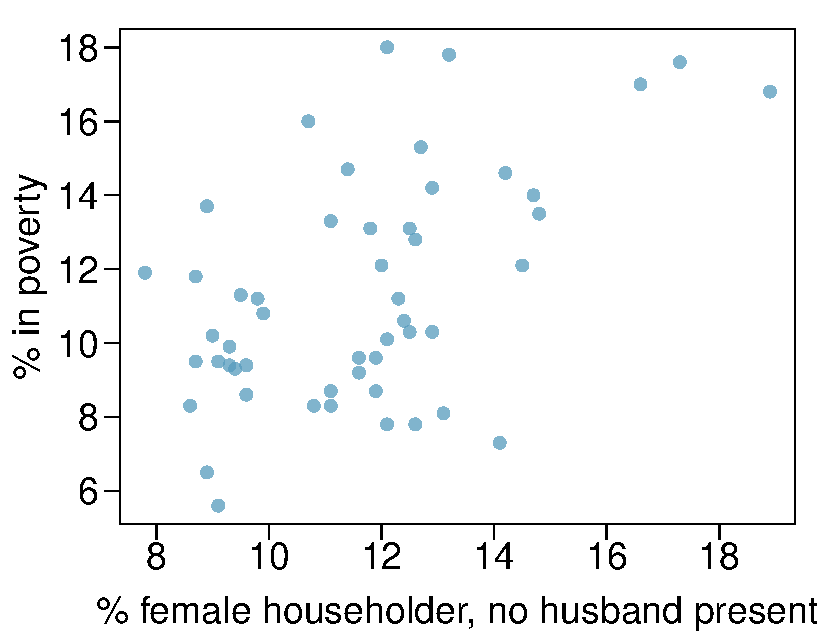
\includegraphics[width=\textwidth]{7-1_linefit_res_corr/figures/poverty/poverty_nohusband}
\end{center}
}

\end{frame}

%%%%%%%%%%%%%%%%%%%%%%%%%%%%%%%%%%

\begin{frame}
\frametitle{Assessing the correlation}

\pq{Which of the following is has the strongest correlation, i.e. correlation coefficient closest to +1 or -1?}

\twocol{0.8}{0.2}
{
\begin{center}
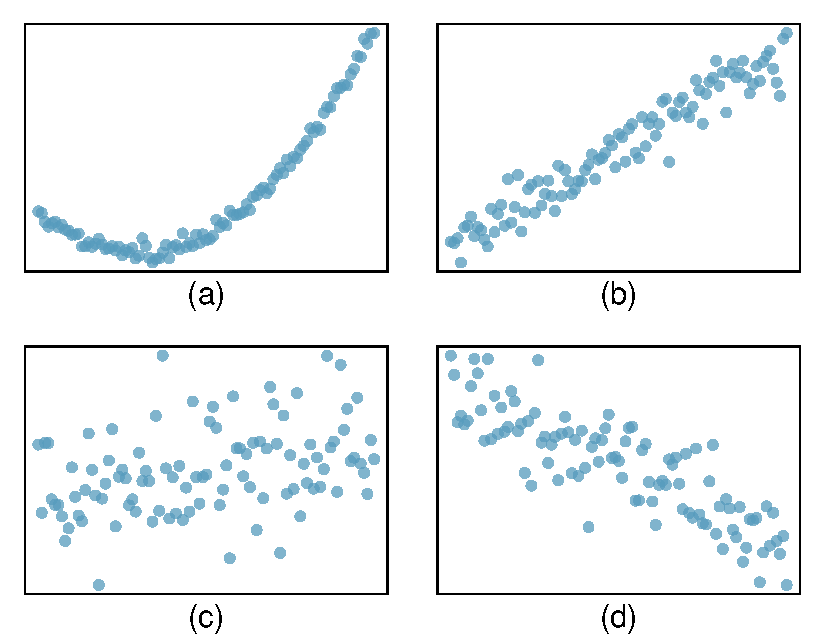
\includegraphics[width=0.75\textwidth]{7-1_linefit_res_corr/figures/cor/cor}
\end{center}
}
{
\soln{\only<2>{\red{
(b) $\rightarrow$ correlation means \underline{linear} association
}}}
}

\end{frame}
